\chapter{Proteus}
\label{chap:methodes}

Il existe plusieurs logiciels de CPD.Parmi les plus connus, On peut citer ORBIT (Optimisation of Rotamers By Iterative Techniques) \cite{Dahiyat96}, OSPREY (Open Source Protein REdesign for You) \cite{Gainza13}, Rosetta (le CPD n'est qu'une partie des fonctionnalités proposés par cette suite logiciel) \cite{Kuhlman03} et Proteus \cite{Simonson13}. Proteus est le logiciel développé par notre équipe au laboratoire de Biologie de l'Ecole Polytechnique. Dans ce chapitre, nous détaillons quelques points importants de notre logiciel.  

\section{Un modèle fondé sur la Physique}
\label{sec:Phy}
Proteus se base sur la théorie de la mécanique statistique pour ses définitions de la stabilité d'un système, de l'affinité entre deux groupes et pour guider sa sélection de meilleures séquences-conformations. A partir d'un postulat fondamental et de l'hypothèse ergodique, la mécanique statistique \og redécouvre \fg la thermodynamique classique et en plus établi une relation à l'équilibre entre l'énergie d'un état $i$ d'un système et la probabilité que le système soit dans l'état $i$ via la probabilité de Boltzmann \ref{eq:Boltzmann}.

Ainsi, si l'on considére deux états A et B d'un système S à l'équilibre, la probabilité que S soit plus souvent dans l'état A que dans l'état B s'exprime comme une différence de l'énergie de A et de B. Pour le CPD, l'énergie qui est pertinante est celle qui prend en compte l'énergie interme de la protéine mais aussi son environement via l'entropie et la température. Il s'agît de l'énergie libre de Gibbs $G$.

Nous introduisons alors un cycle thermodynamique pour définir la stabilité d'une séquence-conformation, voir figure \ref{fig:cycleThermo}.Le cycle considére la stabilité de deux séquences A et B. La transformation de A en B correspond aux deux flèches horizontales. Le dépliement est figuré par les deux flches verticals . La difference de stabilité entre les deux séquences correspond à la différence d'énergie libre des transformations horizontales (comme verticales).

\begin{equation}
  \label{deltaG}
\Delta \Delta G = (G(S^p_B)- G(S^P_A)) - (G(S^D_B)- G(S^D_A))
\end{equation}  
avec $S^p_A$ le système avec la séquence $A$ pliée, $D$ une séquence déplié.

Maximiser la stabilité d'une séquence-conformation correspond alors à minimiser $\Delta \Delta G$.

   \begin{figure}[!htbp]
     \centering
     \begin{tabular}{cc}
       
\includegraphics[width=5cm]{figure/cycleThermo.png} &
     \end{tabular}
     
     \caption{Le cycle thermodynamique qui définit la stabilité}
\label{fig:cycleThermo}
   \end{figure}

On a alors la différence 


\section{Organisation générale}

Proteus est constitué de deux parties:

\begin{enumerate}
\item un ensemble de scripts XPLOR, qui controle le calcul de la matrice d'énergie. (XPLOR est un programme de simulation moléuclaire (\ref{}), disponible en téléchargement sur le site de l'université de Yale).
\item un programme écrit en C ,que nous appelons \og proteus\fg dans la suite de ce texte, qui explore l'espace de sequence/conformation
\end{enumerate}

Le logiciel est flexible et largement configurable; Il permet l'utilisation de plusieurs champ de force, de plusieurs modèle de solvant, et de plusieurs librairie de rotamer.La partie en C, proteus, propose plusieurs algorithme d'exploration comme l'heuristique, MC ou REMC . Le programme proteus permet de diviser le système en plusieurs groupes ou d'en dupliqué une partie , ceux-ci pouvant alors être combiné dans une fonction de score basée sur la fonction d'énergie physique afin de favoriser la stabilité de certains sous-ensembles du système ou certaines affinités.
Plusieurs succès ont déjà était obtenue avec Proteus par exemple de redesign de la tyrosyl-tARN synthetase (\ref{}) ou sur la D-tyrosine ref{}, sur les cacluls de pK_a \ref{31}.

Nous detaillons les points importants de Proteus.

Notre logiciel Proteus autorise le choix entre plusieurs type de fonction d'énergie.Dans le type le plus simple \ogMMCASA\fg, est combinée l'approche de la mécanique moléculaire pour le traitement de la protéine et un modèle de solvant implicite de type CASA (voir  ~\ref{}). Deux types \ogLLGBSA\fg sont égalament possibles , dans lesquels le traitement du solvant est effectuée par un modèle Born Genéralisé.

\section{Décomposition par paires de la fonction d'énergie}
Comme il a était vu précédement, avoir une fonction d'énergie décomposable par paire a plusieurs avantages, en particulier le calcul des énergies des paires de résidues avant l'étape d'exploration permet de reduire le calcul de l'énergie d'une séquence conformation pendant celle-ci à une somme d'énergies pré-calculées. Cependant les termes GB et SA ne sont pas décomposable par paire. Il faut alors introduite de nouvelles approximation pour permettre cette décomposition. Nous allons dans la suite comment ces problèmes sont résolues dans Proteus.
\subsection{Décomposition du terme de surface}
\label{sub:surpairwise}

Le terme surfacique présenté en \ref{eq:SA} ce défini comme:

\begin{equation}
E_{solv}^\surf = \sum_i \sigma_{t_i} A_i 
\end{equation}
avec $A_i$ la surface accessible au solvant de l'atome $i$, et $\sigma_{t_i}$ un coefficient d'hydrophobicité du type de l'atome $i$.
Ce terme n'est pas décomposable par paire de résidu, parce que la surface enfouie d'une première chaîne latérale par une deuxième  peut aussi être enfuie par une troisième chaîne latérale, voir la figure \ref{fig:intersurf}.

   \begin{figure}[!htbp]
     \centering
     \begin{tabular}{c}
       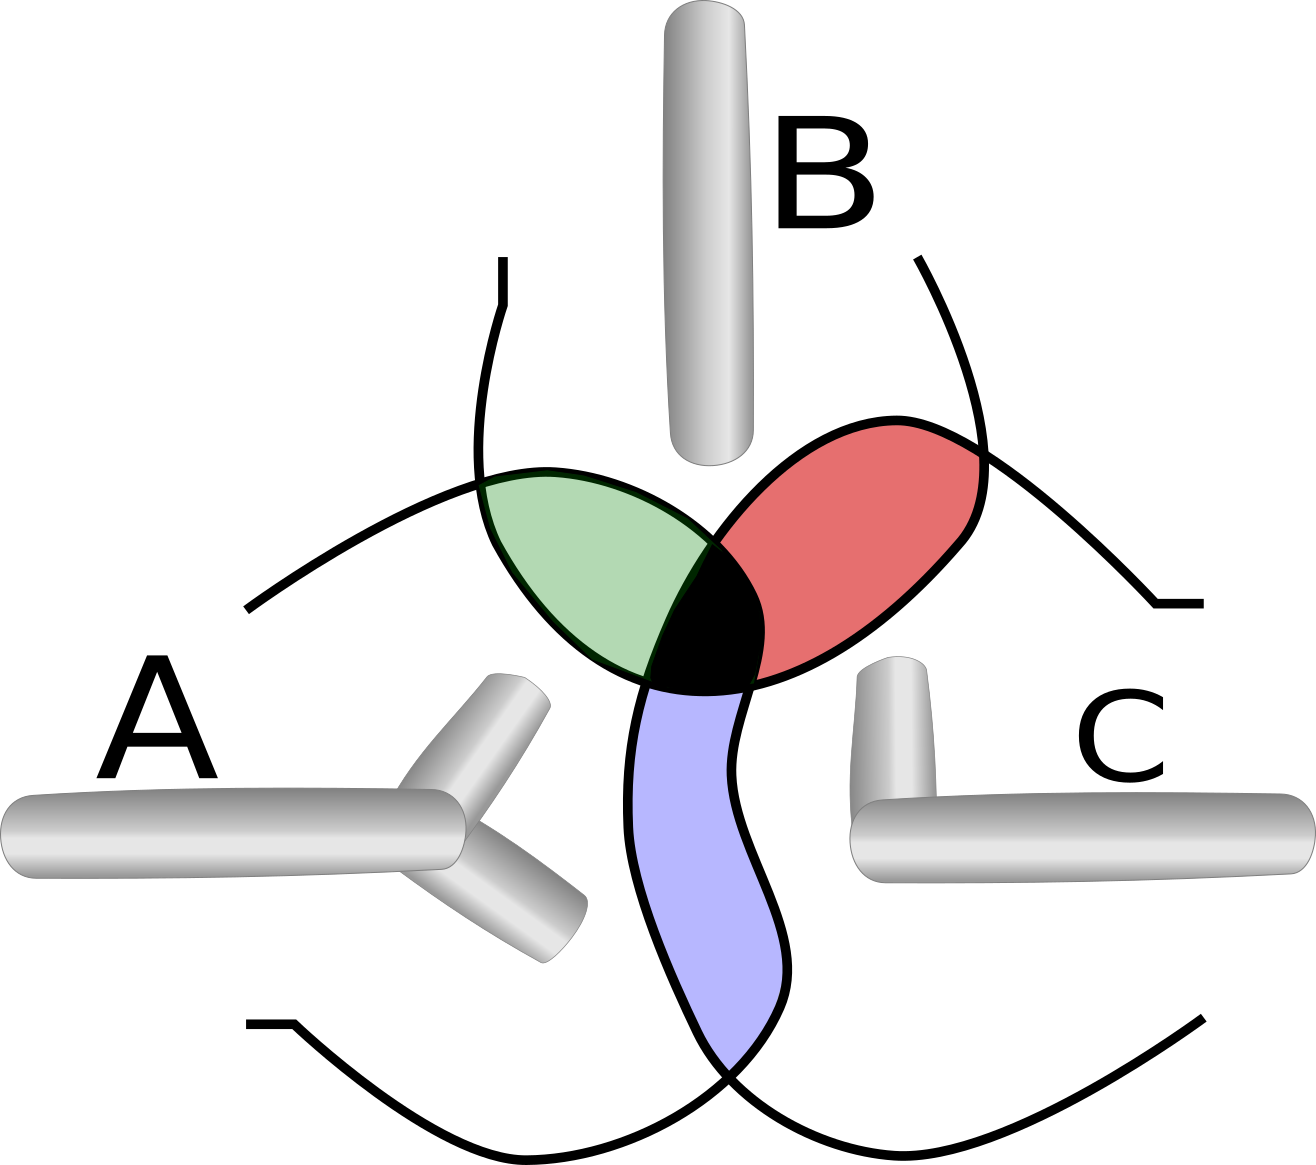
\includegraphics[width=8cm]{figure/intersurface.png} 
     \end{tabular}
     
     \caption{\textbf{Une représentation de la surface accessible de trois résidus} Les résidues A et B réduisent mutuellement leur surface exposée au solvant: c'est la zone verte. De même pour B,C : la zone rouge et  A,C, la zone bleue. Un calcul par paire de résidues naïf surestime la surface accessible en comptant deux choix la zone noire. }
\label{fig:intersurf}
   \end{figure}


Pour rendre ce terme décomposable, nous utilisons la méthode de Street et al. \ref{Street98}, dans laquelle la surface enfuie d'une chaîne est calculée à partir d'une somme sur les chaîne et les groupes du backbone voisins. Puis pour chaque groupe voisins, la zone de contact avec notre chaîne est calculée indépendament des autres groupes. Ces zones sont sommées et un facteur de contraction est appliqué mimant l'élimination des zones comptée à plusieurs reprise. Des travaux précédents effectuée dans notre laboratoire ont montré qu'un facteur de 0,65 fonctionne bien \cite{Lopes07,Gaillard14}.   


\subsection{\og Native Environnement Approximation\fg (NEA)}

Dans le terme GB de l'énergie de solvatation, le rayon de solvatation $b_i$ approche la distance de l'atome $i$ à la surface de la protéine, et donc c'est une fonction de la position relative à $i$ de tous les atomes de la protéine. Et ce rayon n'est pas décomposable par paire. Pour qu'il ne devienne, Proteus implémente l'approximation  NEA qui est présenté à  la section \ref{NEA}, 
Dans cette approche, le rayon de solvatation $b_i$ de chaque groupe (backbone, chaîne latérale ou ligand)  est calculé avant l'étape d'exploration.

\subsection{\og Fluctuating Dielectric Boundary\fg (FDB)}
\label{FDB}
Une nouvelle approximation du GB a récement été introduite dans Proteus \cite{Villa17}, toujours avec l'objectif, de transformer ce terme en en terme additif par paire. Elle exploite le fait que dans le GB, l'environement dielectrique  d'une paire de résidue est completement caractérisé pour un petit ensemble de rayon de solvatation d'atome. Ces rayons sont eux-mêmes sommes de paires sur les atomes de la protéine \cite{Hawkins95}, \cite{Schaefer96}. La méthode s'appelle Fluctuating Dielectric Boundary\fg ou FDB et comporte les deux étapes suivantes:

La premiere consiste à définir un rayon de solvatation $B_I$ pour chaque résidu $I$ de la protéine.

On commence par définir une énergie propre à chaque paire de résidus I,J par la somme suivante:

  \begin{equation}
    E_\IJ^{self} = \sum_{i\in I,j\in J} E_\ij^\self
  \end{equation}
  puis l'énergie propre d'un résidu I:

  \begin{equation}
    E_\I^{self} = \sum_J E_\ij^\self
  \end{equation}
    
  Alors le rayon de solvatation moyen $B_I$ est défini par:
\begin{equation}
    E^{self}_I \stackrel{def}{=} \tau \sum_{i \in I} \frac{q_i^2}{2 B_I}.
\end{equation} 

Nous avons, alors

\begin{equation}
\left( \sum_{i \in I} q_i^2 \right) \frac{1}{B_I} = \sum_{i \in I} \frac{q_i^2}{b_i}.
\end{equation}

Donc, $B_I$ est la moyenne harmonique des $b_i$, avec $i \in I$, pondéré par les charges au carré.

Il et alors possible de définir la contribution $g_\IJ$ de la paire de résidu I et J à l'énergie d'écrantage total $\Delta^\solv$, par:

\begin{equation} 
g_{IJ} = \sum_{i \in I, j \in J} \tau q_i q_j \left( r_{ij}^2 + B_I B_J \exp[-r_{ij}^2/4 B_I B_J] \right)^{-1/2}
\label{eq:screen}
\end{equation}

avec, la somme pour $I=J$ excluant le cas $i \neq j$.
On peut noter qu'aux distances fixes $r_\ij$, et avec $B=B_IBJ$, $ g_\IJ (B)$ varie faiblemement en fonction de B. Archontis et Simonson \cite{Archontis05}, proposent alors d'approximer cette fonction par:

\begin{equation}
  \label{eq:approx}
g_{IJ}(B) \approx c_1^{IJ} + c_2^{IJ} B + c_3^{IJ} B^2 + c_4^{IJ} B^{-1/2} + c_5^{IJ} B^{-3/2}  \label{eq:approx}
\end{equation}

Les coefficients $c_n^{IJ}$ peuvent alors être pré-calculé est stocké dans la matrice d'énergie, puisque les distances $r_\ij$ ne sont pas des variables pour un couple de chaîne latérale I,J donné. 
Comme les rayons de solvatation d'un résidu sont eux-mêmes des sommes sur les paires, le calcul de l'énergie GB à l'aide de \ref{eq:approx} est maintenant décomposable par paire.



\section{La matrice d'énergie}

Proteus utlise d'une part un backbone fixe, une espace discrét de rotamère et une fonction d'énergie décomposable par paires. Ces trois élèments permettent de pré-calculer toutes les énergies interactions possibles. A cet ensemble d'interactions, il faut ajouter les interactions des résidues avec le backbone ceci pour chacun des rotamères possibles, pour constituer un ensemble complet de valeur énergétiques qui permet d'obtenir la valeur de la fonction d'énergie pour chaque sequence/conformation. Cet ensemble peut être organisée sans le format d'une matrice symétrique dans laquelle chaque couple de position dans la chaîne polypeptidique, apparait avec sa multiplicité de couples de rotamères possibles voir ~\ref{Graph:mat_ener}.      


   \begin{figure}[!htbp]
     \centering
     \begin{tabular}{c}
       
\includegraphics[width=15cm]{figure/matrice.png}
       \label{Graph:mat_ener}
     \end{tabular}
     
     \caption{\textbf{La matrice d'énergies} Sur cet exemple, un polypeptide de 6 résidues, chaque position posséde type d'acide aminés possibles et 3 rotamères possibles (2 pour le type A et 1 pour le type B). La matrice organise toutes les interactions de paires de chaîen latérales possibles. Les interactions impliquant le résidu numéro 2 sont dans la bande jaune de la matrice, les interactions impliquant le résidu numéro 3 sont dans la bande bleue. Les points rouge et vert correspondent aux interactions  noté par les flèches rouge et verte à gauche(La matrice est symétrique , ici les interactions sont reprrésentées qu'une seule fois).}
\label{graph:MAt_ener}
   \end{figure}
   

\subsection{Les énergies de l'état déplié}

le $\Delta \Delta G$ s'applique entre l'état replié de la protéine et un état déplié. Nous avons donc besoin d'attribuer une énergie à l'état déplié. Proteus exploite une definition indépendante la structure telle que:
\begin{equation}
E_u(S) = \sum_i^N E(t_i)  
\end{equation}

avec $E(t_i)$ une énergie du type d'acide aminé $t_i$.

Ces énergies sont prises en entrée dans Proteus, et donc sa détermination ne fait pas encore partir des fonctionnalité intégré à notre logiciel. Il apparaît clairement dans la suite que la détermination doit être fonction du système étudié. Nous detaillerons dans le chapitre \ref{chap:PDZ}, plusieurs méthodes dont de nouvelles et plusieurs exemples de détermination qui seront exploités et évalués.


\subsection{Déroulemement de la construction de la matrice}
\label{sub:matrix}

Dans la suite, on appelle \og position active \fg, une position pour laquelle, tous les types d'acides et tous les rotamères de chaque type d'acide aminé sont autorisés, au court de la recherche de proteus.

Lorsqu'une position n'est pas active, l'acide aminé de la position est fixé en utilisant l'acide aminé de la séquence native. Si la chaîne latérale n'est pas fixé on dit que la position est \og inactive\fg. Si la position n'est pas active et qu'en plus la chaîne latérale est fixé on dit que la position est gelée.

Le calcul de la matrice d'énergie, sont executer à l'aide du programme X-plor \cite{Brünger92}. il se déroule de la façon suivante:
A partir d'un fichier PDB, une série de script XPLOR va préparer le système. Il peut contenir un ligand.

\begin{enumerate}
-1- L'utilisateur configure l'execution:
Il determine:
\begin{itemize}
\item un champ de force. Les champs AMBER ff99SB ou CHARMM toph19 sont tous les deux supportés.
\item un traitement de l'électrostatique du solvant parmi CA GB/NEA GB/FDB
\item un jeu de coefficients $\sigma_i$ pour la pondération de la surface accessible au solvant dans le terme hydrophobe.
\item l'ensemble des résidus dans le backbone autorisé à muter
\item l'ensemble des chaînes laterales autorisé à se déplacer 
\end{itemize}

-2- Les atomes du squelette sont fixés une fois pour toute.

-3- Pour chaque résidu, les atomes des chaînes latérales sont placés avec les angles dièdres issue de la bibliothèque de rotamères. L'ensemble de conformation ainsi défini est sauvegardé dans un fichier PDB par position.

-4- Les rayons de solvatation de Born sont calculé selon l'approximation GB demandé. Ces rayons sont sauvegardé dans un fichier dédié.

-5- Pour chaque rotamére de chaque type, après une petite minimisation, où lui seul peut se déplacer, l'énergie d'interaction avec le squelette est calculée. Elle est stocké dans une fichier. Ce sont les énergies de la diagonale de matrice. l'objectif de la minimisation est d'adapter le rotamère à son environement natif.

-6- Pour chaque paire de rotamère possible,comme pour la diagonale de ma matrice, une petite minimisation est effectuée avec uniquement la paire courante qui peut se deplacer. Puis les termes d'énergie d'interaction du couple sont  calculés et enregistrés dans du fichiers.  
\end{itemize}

Pour chaque paire d'acides aminés, l'énergie d'interaction a été obtenue après 15 pas de minimisation de l'énergie, seules les interactions de la paire entre les autres chaînes et le backbone sont prises en compte. Cette courte minimisation simplifie l' approximation discrète. Les rotamères de chaînes latérales utilisés sont une version légèrement étendue de la librairie de Tuffery et al. \cite{Tuffery91}, qui possède un total de 254 rotamères (sur l'ensemble des types d'acides aminés).Cette extension comprend des orientations d'hydrogène supplémentaires pour les groupes OH et SH \cite{Gaillard14}. Cette bibliothèque de rotamères a été choisie pour sa simplicité et parce qu'elle a donné de très bonnes performances dans les tests de placement de chaînes en comparaison au programme spécialisé scwlr4 qui utilise une bibliothèque beaucoup plus grande \cite{Krivov09,Gaillard16}.

Les scripts sont concus pour pouvoir distribuer les calculs sur différentes architectures matérielles allant du PC mono- processeur au cluster de calculs hétérogènes.

\subsection{les fichiers d'énergies}

Après Le calcul de la matrice d'énergies, une étape de fusion des résultats obtenus permet d'obtenir deux fichiers d'énergies : un fichier d'énergies propres et un fichier d'énergies d'interactions.

Le premier rassemble les énergies propres de chaque chaîne latérale possible et l'énergie d'interaction de cette chaîne avec la partie fixe de la protéine c'est-à-dire le backbone et les résidus non modifiables dans le système étudié. Chaque ligne de ce fichier correspond à un rotamère possible de chaque chaîne latérale possible de chaque position non fixée. Les quatres premiers champs identifie la position du résidue, son type, son rotamère. Les autres champs contients les termes de l'énergie. Le nombre de ces termes variant selon le traitement du solvant, les détailles sont montrés aux figures \ref{fig:CAenerfile} et \ref{fig:GBenerfile}.   
Le second fichier rassemble les énergies entre les paires de rotamères. Il comporte deux types de lignes. Le premier donne le couple de position et le couple de type d'acide aminé considérés. des lignes du second type suivent une ligne du premier type et donne dans les deux premier champ le couple de rotamères impliqué dans l'interaction.Suivent alors l'ensemble des termes énergétiques de l'interaction, \ref{fig:CAenerfile} et \ref{fig:GBenerfile}. 


Ensuite , les differents fichiers d'énergies seront lu par proteus voir \ref{} 


   \begin{figure}[!htbp]
     \centering
     \begin{tabular}{c}
       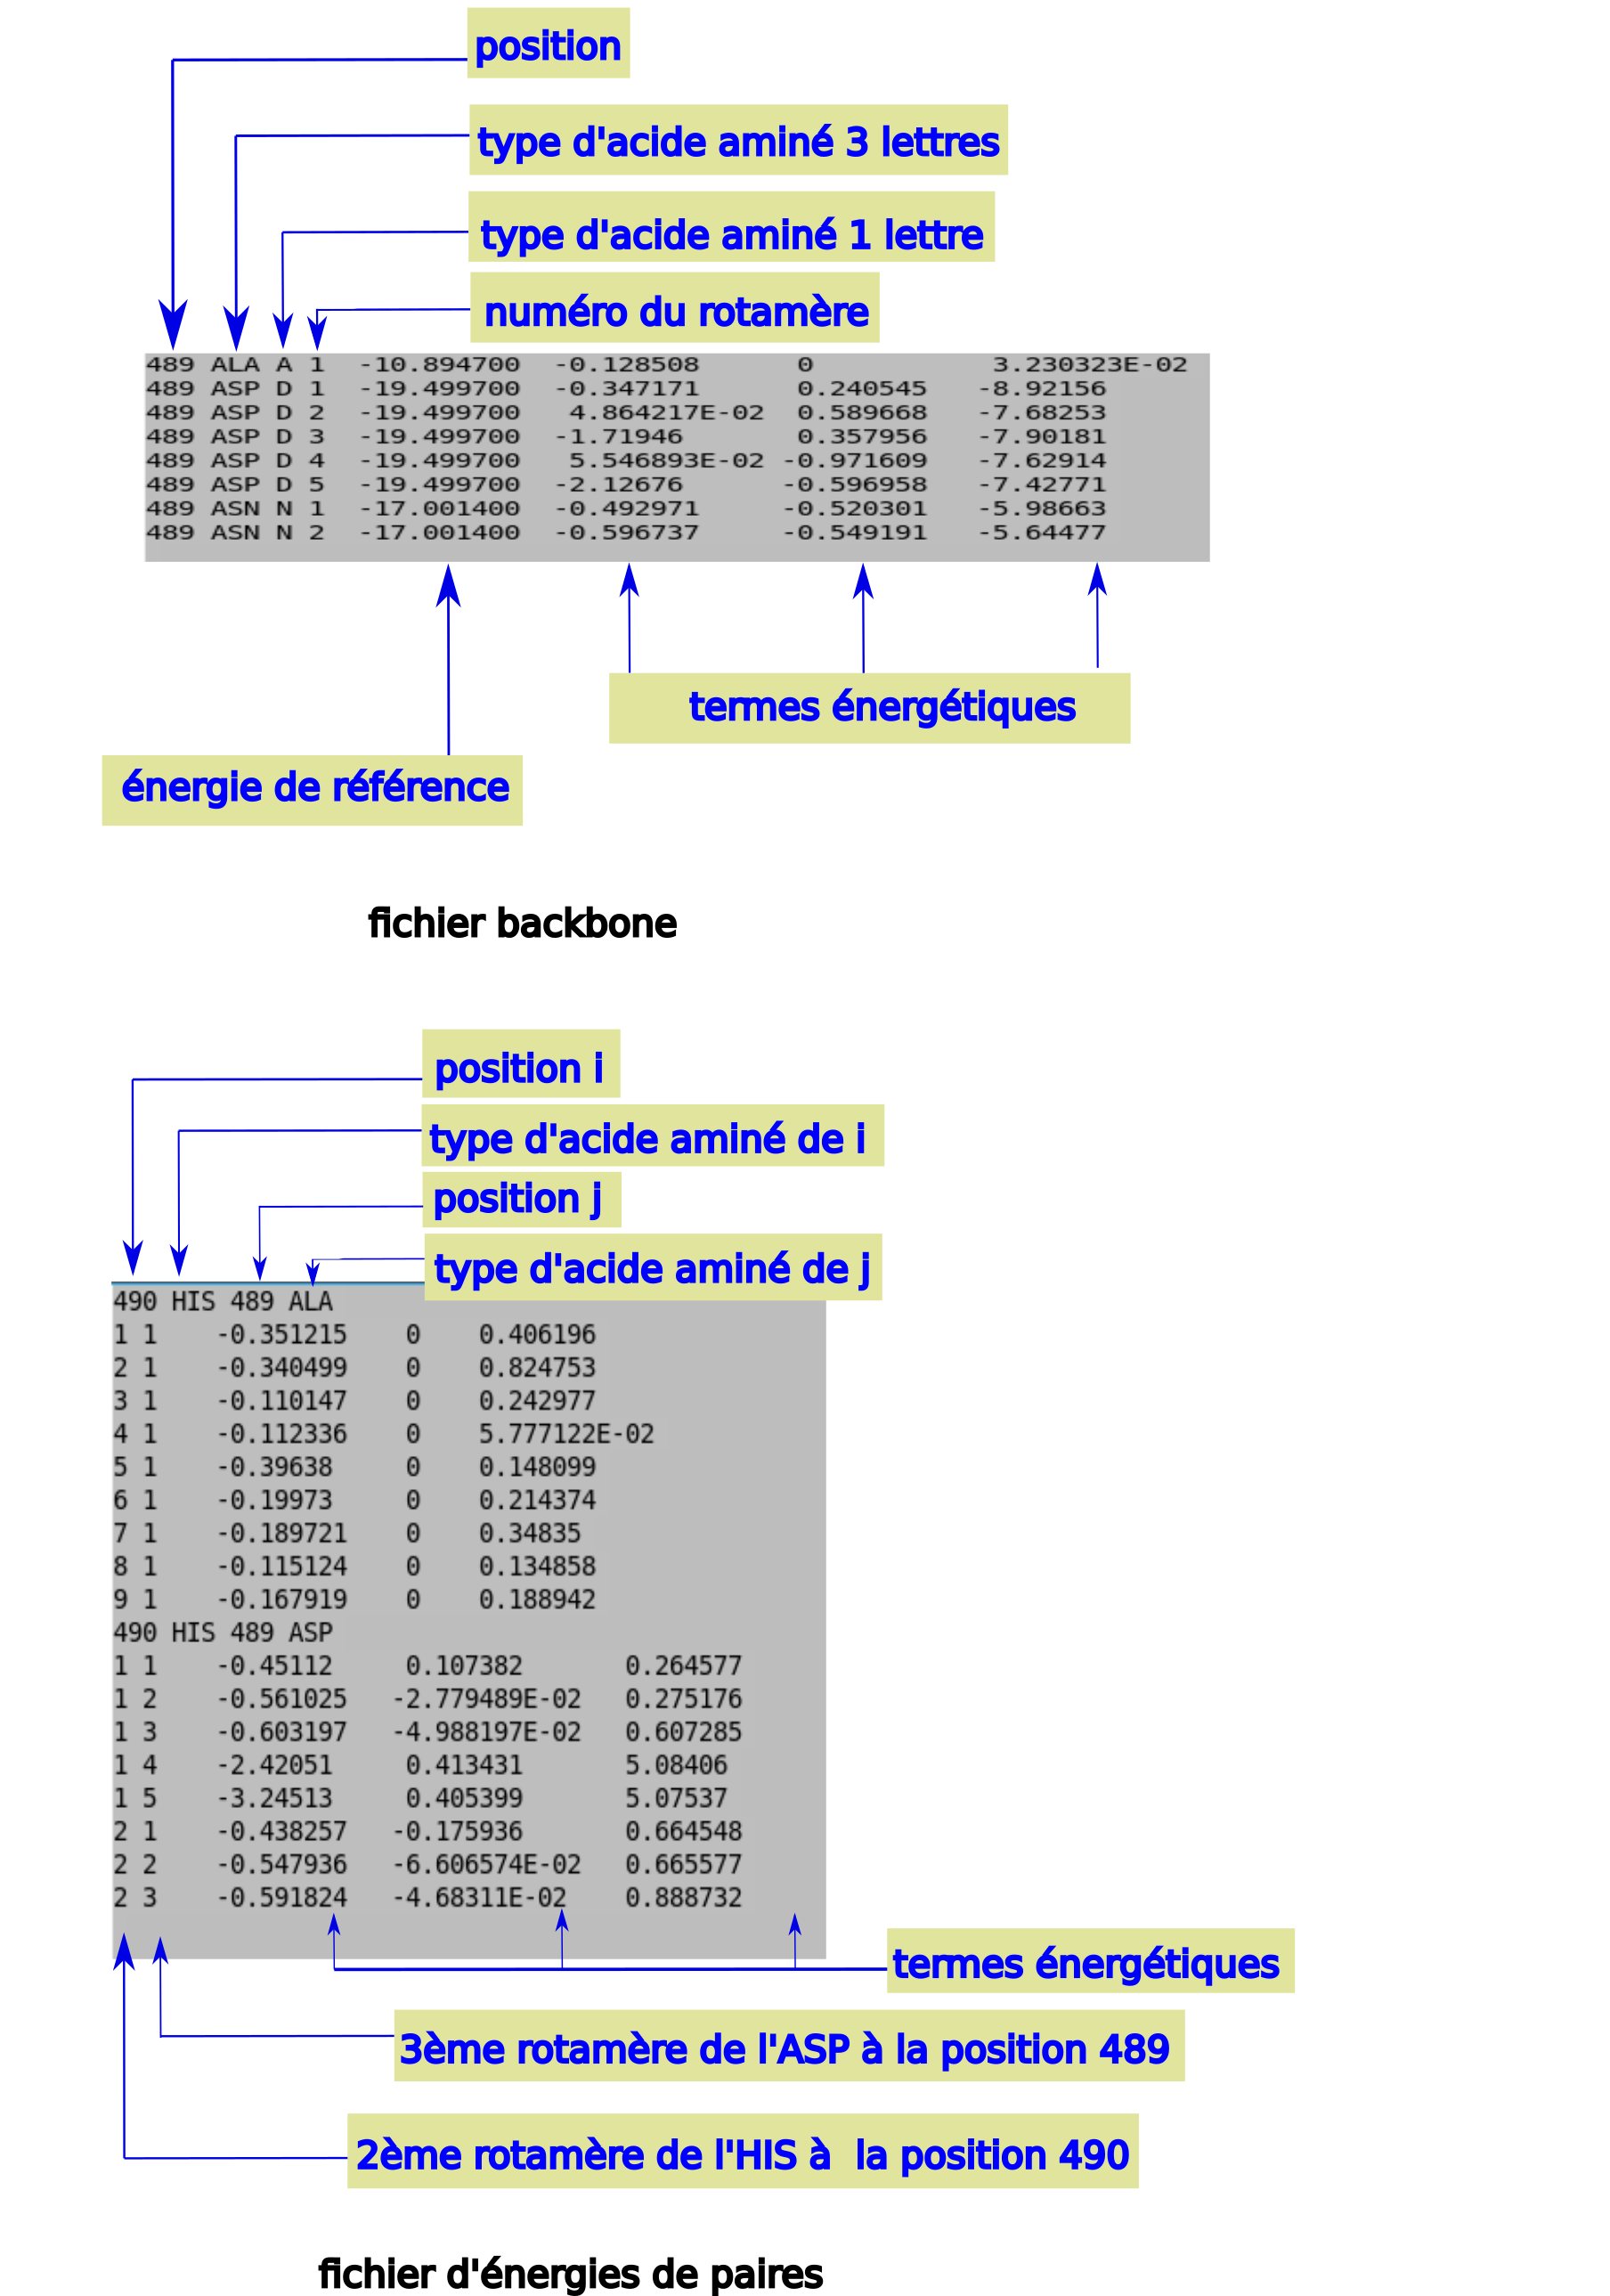
\includegraphics[width=12cm]{figure/inputener.png} 
     \end{tabular}     
     \caption{\textbt{Les fichiers d'énergies en mode CA}}
\label{fig:CAenerfile}
   \end{figure}


   \begin{figure}[!htbp]
     \centering
     \begin{tabular}{c}
       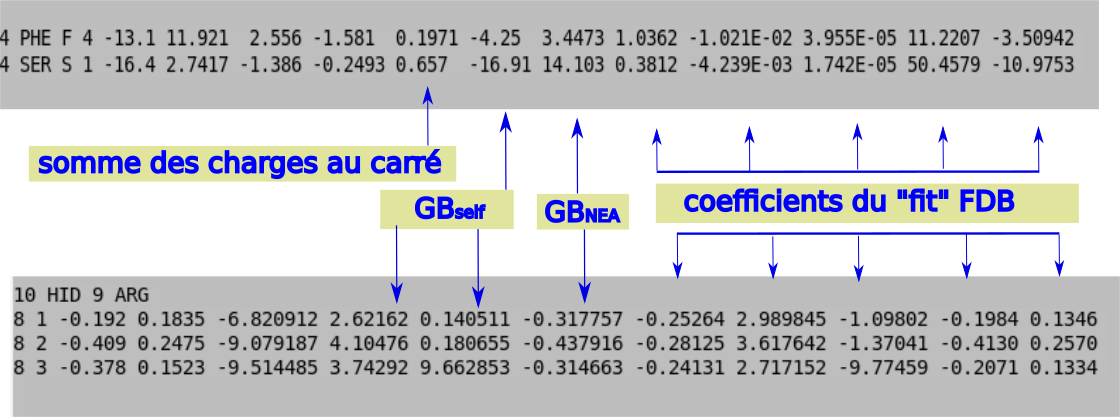
\includegraphics[width=12cm]{figure/inputenerGB.png} 
     \end{tabular}     
     \caption{\textbt{Les fichiers d'énergies en mode GB NEA et FDB}}
\label{fig:GBenerfile}
   \end{figure}
   

\section{Configuration de l'exploration}

L'étape suivante est l'exploration à l'aide des énergies obtenues. Elle s'effectue avec le programme proteus écrit en C. Ce programme se contrôle par une fichier de configuration de type XML sans imbrication de balise, Il y a actuellement près de quarante balises possibles, une partie est présentée table \ref{tab:balise_proteus}. Nous en détaillons quelques unes ici.

L'utilisateur peut choisir la méthodes d'exploration (MSD, MC/REMC ou champ moyen).

Pour le MSD, il peut paramètrer le nombre de cycle et le nombre de passage sur la séquence, voir section \ref{MSD}.
Pour le MC/REMC, le fichier de configuration détermine le nombre de marcheurs, la taille de chaque trajectoire, la période de \og swap \fg, c'est-à-dire la période, en nombre de pas, à laquelle une tentative d'échange de répliques est effectuée ( voir \ref{REMC_move} ) (si elle est non-nulle, l'exploration est de type REMC).

Pour controler les déplacements des marcheurs, il existe 
\begin{itemize}
\item un ensemble de cinq  balises pour définir les modifications à effectuer dans la séquence-conformation courante, voir le chapitre \ref{chap:developpement}
\item une balise qui definit un voisinnage de la première position modifié dans lequel sera choisi une autre position pour une seconde modification, voir la section \ref{sub:MC_move}.
\end{itemize}

Il est possible de réduire l'espace des états que peut prendre une séquence-conformation. Les explications sous en \ref{sub:restric}.Il existe deux balises pour définir un système de groupes et déclarer une fonction de score. Ceux-ci permettent de définir une optimisation non plus uniquement du type de l'équation \ref{deltaG}, mais répondant un ensemble de problématique nettement plus large. Nous détaillons ce système  en \ref{sub:group} et \ref{sub:score}.

    \begin{table}[!htbp]
      \centering

      \begin{tabular}{|p{0.2\linewidth}|p{0.35\linewidth}|p{0.45\linewidth}|}

        \hline
        Type   & nom & Description \\
        \hline
          methode  d'exploration & Mode &  determine  le mode d'exécution, les valeurs possibles sont HEURISTIC(MSD),MONTECARLO,MEANFIELD et POSTPROCESS  \\  \hline    
                        & Trajectory\_Length  &  la longueur de la trajectoire MC ou REMC\\  \cline{2-3}
        nombre de pas & Trajectory\_Number  &  le nombre de trajectoire  MC ou REMC  \\  \cline{2-3}
                        & Cycle\_Number  &    le nombre de cycle en mode HEURISTIC   \\ \cline{2-3}  
                        & Sequence\_Pass\_Number  &  le nombre maximum d'iteration sur  la structure à chaque cycle(mode HEURISTIC)    \\ \hline  

        fonction d'énergie &  Optimization\_Configuration &   definition de la fonction d'énergie\\               \cline{2-3}
                        &  Group\_definition &   groupes  d'energies et d'énergies d'interactions,ce sont les éléments de base de la fonction d'énergie\\  \hline  
        restrictions de l'espace de  sequence/rotamer & Space\_Constraints   &  restraint les états visités \\ \hline                
                         
     paramètre du modèle & Temperature & attribue les températures aux marcheurs MC  \\          \hline     
                         & Random\_Generator &  Le générateur de nombre aléatoire de la \og GNU Scientific Library \fg \\ \cline{2-3}
                         & Rot\_Proba &  probabilité d'avoir un changement de rotamère à chaque pas \\              
        Configuration    & Rot\_Rot\_Proba &  probabilité d'avoir un double changement de rotamère à chaque pas\\          
        Monte Carlo      & Mut\_Proba &  ... \\              
                         & Mut\_Mut\_Proba & ... \\              
                         & Mut\_Rot\_Proba & ... (ancienne version de Proteus)\\             \cline{2-3}  
                         & Position\_Weights  & probabilité de tirage de chaque position, lors de la première choix\\  
                         & Step\_Definition\_Proba  & probabilté de changer un rotamère ou un type d'aa\\   \cline{2-3}
        
                         & Neighbor\_Threshold & à chaque pas les changement se font dans le même voisinnage énergétiques.Cette balise définit la taille des voisinnages.\\   \hline
        
                         & Fasta\_File & le nom du fichier produit par le mode POSTPROCESS\\    \cline{2-3}             
        Input/Output     & Seq\_Output\_File & le nom  du fichier de séquences produit par le mode HEURISTIC ou MONTECARLO\\    \cline{2-3}             
                         & Energy\_Output\_File & le nom du fichier d'énergie produit par le mode  HEURISTIC ou MONTECARLO\\   \hline              

      \end{tabular} 

      \caption{ Une partie des balises possibles dans le fichiers de configuration de Proteus}      

      \label{tab:balise_proteus}

  \end{table}

\subsection{Les déplacements Monte-Carlo}

\label{sub:MC_move}

Dans l'algorithme de metropolis, il est nécessaire de définir une probabilité de sélectionner un état $B$ lorsque le système est dans l'état $A$. Pour proteus, une transition se définit par des modifications à certaines positions de la séquence-conformation courante. Il y a deux types de modification élémentaires: une mutation et un chagement de rotamère qui peuvent être combinés. Cinq balises permettent de définir des probabilités associées à ces modifications:

\verb!<Rot_Proba>! \\
\verb!<Mut_Proba>! \\
\verb!<Rot_Rot_Proba>! \\
\verb!<Mut_Rot_Proba>! \\
\verb!<Mut_MuT_Proba>!  \\
chacune prend en paramètre une valeur comprise entre $0$ et $1$. Les deux premières fixent la probabilité des deux modifications élémentaires. Les trois autres fixent la probabilité de modifier deux positions simultanement, c'est à dire au court du même pas Monte-Carlo.
Le choix d'un première position à modifier se fait toujours par tirage aléaoite sur l'ensemble des positions du système. En revanche, le choix de la seconde position à modifier se fait par tirage aléatoire dans le voisinnage de la première position. Le voisinnage d'une position se définit de la façon suivante.

Deux positions $i$ et $j$ sont voisines s'il existe un rotamère $r_i$ de $i$ et un rotamère $r_j$ de $j$ tels que:
\begin{displaymath}
  \label{\ref{para:voisin}}
 | E(r_P_i_,r_p_j) | > s_{vois}
\end{displaymath} 
avec $s_{vois}$ le seuil donné par l'utilisateur dans la balise \verb!!.
Le voisinnage d'une position $i$ est l'ensemble de ses voisins.


Ce système de déplacements MC a été revu pendant ma thèse, voir section \ref{}.

\subsection{Restriction de l'espace séquence-conformation}
\label{sub:restric}

Dans proteus, l'espace des états possibles se définit par le contenue du fichier \og backbone \fg. Cependant, l'utilisateur a la posibillité de restrainte cet espace sans modification des fichiers d'énergie. Il peut le faire un utilisant la balise \verb!<Space_Constraints>! de la façon suivante:

\verb!<Space_Constraints>! \\
\verb!489  LYS TRP! \\
\verb!490  ASN ARG{1,8,12}! \\
\verb!</Space_Constraints>! \\

Cela signifie qu'à la position 489 seules les types LYS et TRP sont possibles et qu'à la position 490, les deux types ASN et ARG sont possibles, mais que pour ARG seule les rotamères 1 , 8  et 12, selon l'indexation fourni dans fichier \og backbone \fg, sont autorisés. Cette balise permet d'autres classes de restrictions qui sont exposées plus loin.

 \subsection{Définition de la fonction de score }

 Le cycle thermodynamique \ref{fig:cycleThermo} peut être adapter pour exprimer d'autres problèmatiques que celle de la recherche de séquences stables. C'est le cas des calculs de $pK_a$ par l'expression d'une différence d'énergie libre de protonation. La problèmatique CPD de la reconnaissance d'un ligand par une protéine peut également être traitée. Cela peut se faire par un critère d'affinité via l'énergie libre d'interaction ou par un critère de spécificité. Le critère d'affinité se base sur le cycle thermodynamique  \ref{fig:cycleThermoLignad} qui permet d'écrire l'équation:

 \begin{equation}
   \label{deltaG2}
\Delta \Delta G = (G(P:L_2)- G(P:L_1)) - (G(L_2) - G(L_1))
\end{equation}  
avec $P$ la protéine,$L_1$ et $L_2$ deux ligands et $P:L_i$ un complexe protéine-ligand. 
Cette expression suppose que $P$ se relaxe de la même façon dans les états dissociés des deux complexes. 

   \begin{figure}[!htbp]
     \centering
     \begin{tabular}{cc}
       
\includegraphics[width=5cm]{figure/cycleThermoLigand.png} &
     \end{tabular}
     
     \caption{Le cycle thermodynamique qui définit l'affinité.}
\label{fig:cycleThermoLigand}
   \end{figure}

Le critère de spécificité combine une augmentation de l'interaction avec de nouveaux ligands et une dégradation de l'interaction avec le ligand naturel.

Proteus permet l'utilisation de ce type de critère via la décomposition des équations \ref{deltaG} et \ref{deltaG2} en contribution intramoléculaire et intermoléculaire et autorise une pondération des differents termes. Il pemet de duplicer des parties du système, ouvrant la voie à des optimisations simultanées de deux conformations d'un sous-système à séquences identiques, mais non fixées.   

Nous détaillons maintenant la façon dont ce dispositif fonctionne.

\subsubsection{Définition de groupes}
\label{sub:group}
L'utilisateur a la possibilité de définir des groupes sur le système étudier. Un groupe est associé à une partie du système. Il se définit en donnant la liste des positions qu'il contient dans la balise \verb!<Group_Definition>! du fichier de configuration. Par exemple:

\verb!<Group_Definition>! \\
\verb!grp1 1−3! \\
\verb!grp2 4 5! \\
\verb!grp3 6-8! \\
\verb!</Group_Definition>! \\

Chaque groupe représente une conformation-séquence de sa partie. Il est possible de définir plusieurs groupes associés à un même ensemble de position:

\verb!<Group_Definition>! \\
... \\
\verb!grp3 6-8! \\
\verb!grp4 6-8! \\
\verb!</Group_Definition>! \\

Dans l'exemple précédent le groupe grp4 représente une seconde conformation-séquence des résidus compris entre les numéros 6 et 8 du fichier backbone. Ces conformations-séquences possède toutes deux leur propre espace d'états. L'utilisateur peut les reduires differements l'un de l'aute:


\verb!<Space_Constraints>! \\
\verb!grp3.6  LEU TRP! \\
\verb!grp4.6  ASN ARG!  \\
\verb!</Space_Constraints>! \\

Il peut au contraire relier leurs états respectifs:

\verb!<Space_Constraints>! \\
\verb!grp4.TYPE grp3! \\
\verb!</Space_Constraints>! \\

La déclaration précédente garantie que les groupes grp3 et grp4 auront des séquences identiques tout au long de l'exploration. 

En tirant partie de la décomposition par paires de la fonction d'énergie, il est possible d'exprimer simplement l'énergie d'un groupe et l'interaction entre deux groupes. On a:

\begin{equation}
E(grp_i) = \sum_{a \in grp_i} E_i + \sum_{a \neq b, \in grp_i} E_{a,b}
\end{equation}

et

\begin{equation}
E(grp_i,grp_j) = \sum_{i \in grp_i} E_i + \sum_{i \neq j, \in grp_i} E_{i,j}
\end{equation}


avec $E(grp_i)$ l'énergie du groupe $grp_i$ ,$E(grp_i,grp_j)$ l'énergie d'interaction entre les groupes $grp_i$ et $grp_i$, $E_a$ l'énergie propre du résidu à la position $a$, et $E_{a,b}$ l'énergie d'interaction entre les rotamères aux positions $a$ et $b$.

Il est possible de visualiser les énergies de groupes sur la matrice d'énergies, voir \ref{fig:matrix_grp}. Les contributions à l'énergie d'un groupe se situent dans un carré sur la diagonale de la matrice et les contributions à l'énergie d'interaction entre deux groupes se situent dans un rectangle hors de la diagonale.


   \begin{figure}[!htbp]
     \centering
     \begin{tabular}{cc}
       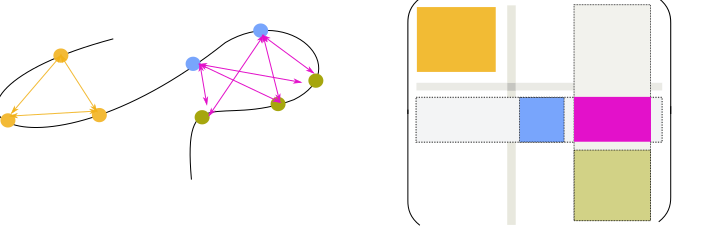
\includegraphics[width=12cm]{figure/grp_matrix.png} &
     \end{tabular}
     
     \caption{\textbf{Les repartitions des contributions aux énergies de groupes et d'interaction entre groupes dans la matrice d'énergie} L'énergie des groupes orange bleu et vert est la sommme de termes des carrés de même couleur dans la matrice d'énergie. L'interaction entre le groupe bleu et le groupe vert est la somme de tous les termes du rectangle rouge.}
\label{fig:matrix_grp}
   \end{figure}
   

\subsubsection{Déclaration de la fonction de score}
\label{sub:score}
Il est alors possible d'introduire une nouvelle matrice qui rassemble les énergies de groupes et les énergies d'interaction entre les groupes, voir la figure \ref{fig:group_matrix}. Dans cette petite matrice l'énergie propre d'un groupe est sur la diagonale, celles d'interaction hors de la diagonale.



   \begin{figure}[!htbp]
     \centering
     \begin{tabular}{cc}
       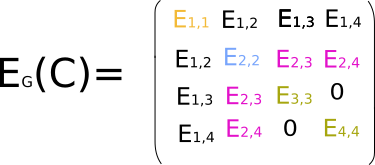
\includegraphics[width=8cm]{figure/group_matrix.png} &
     \end{tabular}
     
     \caption{\textbt{La matrice des énergie de groupe} Les énergies des groupes grp1, grp2, grp3 et grp4 et leurs interactions présentées sont forment de matrice. Il n'y a pas d'interaction entre grp3 et grp4 parce qu'ils sont associés à une même partie du système.}
\label{fig:group_matrix}
   \end{figure}

La fonction de score peut se définir alors comme une combinaison linéaire des élèments de cette matrice. Pour cela il fait utiliser la balise  \verb!<Optimization_Configuration>!:



\verb!<Optimization_Configuration>! \\
\verb!m(0.2grp1+0.2grp2+0.3grp2~grp3-0.3grp2~grp4)! \\
\verb!</Optimization_Configuration>! \\


ici la notation de l'énergie entre deux groupes \verb!grp2! et \verb!grp3! est \verb!grp2~grp3!, et  l'énergie propre d'un groupe \verb!grp1! simplement \verb!grp1!. Les nombres sont des pondérations des énergies. La notation \verb!m(E)! indique que la fonction de score demandée est une minimisation de la somme déclarée entre les parenthèses. Cela signifie que pour deux séquences-conformations A et B, A est meilleure que B si $E(A) < E(B)$.


Il est également possible d'utiliser \verb!t(...)! pour indiquer une fonction de seuil:

\verb!<Optimization_Configuration>! \\
\verb!t(grp1)<125.8! \\
\verb!</Optimization_Configuration>! \\

Ici A est meilleure que B si $E(A)<125,8$. C'est utile dans le cas d'une utilisation de l'algorithme MSD, cela elle permet d'obtenir un ensemble de conformations-séquences avec une énergie inférieur à un seuil.


\section{Les fichiers de sortie}
   
   \begin{figure}[!htbp]
     \centering
     \begin{tabular}{cc}
       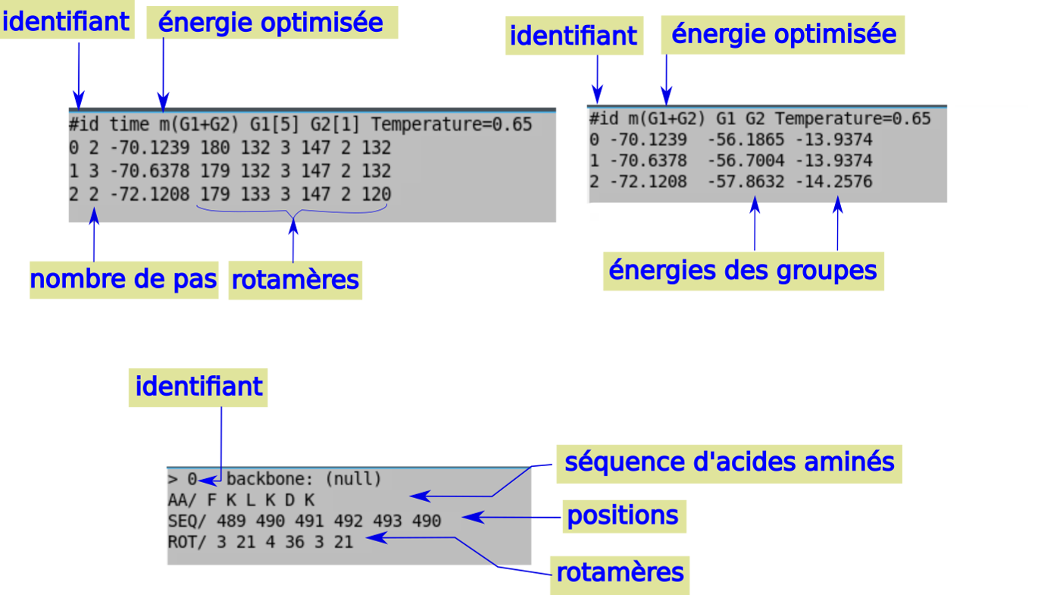
\includegraphics[width=12cm]{figure/output.png} &
     \end{tabular}
     
     \caption{Les fichiers en sortie de proteus}
\label{graph:struct_Phy}
   \end{figure}
   


\section{Outils d'analyse de séquences} 
\subsection{Superfamily/SCOP}
\label{subsection:Superfamily}

Superfamily~\citep{refSuperfamily} est un ensemble composé: 

\begin{itemize}
\item D'une base de données de modèles de Markov cachés, où chaque modèle représente une structure 3D d'un domaine de la classification SCOP.
\item D'une série de scripts qui annotent à partir des informations de la base,les séquences données en entrée. Ici, nous utilisons uniquement l'association au modèle 3D le plus vraisemblable. 
\end{itemize}

Nous travaillons avec la base de données à la version 1.75, et en conjonction, nous utilisons SAM (version 3.5)~\citep{refSam} et HMMER (version 3.0)~\citep{refHmmer} recommandés par l'équipe de Superfamily. Le paramétrage utilisé est celui par défaut. La base SCOP contient 15 438 modèles.

\subsection{Taux d'identité de séquences}

Soient $S$ et $N$ deux séquences d'acides aminés de même longueur $l$.

Le Taux d'identité $Id(S,N)$ de $S$ par rapport $N$ est égal au pourcentage de position où l'acide aminé est identique dans $S$ et $N$. C'est-à-dire:
\begin{equation}
Id(S,N) =\frac{1}{l}\sum_{1<i<l} \mathds{1}(s_i,n_i)} \times 100
\end{equation}
avec $s_i$ et $n_i$ l'acide animé en $i$ de $S$ et de $N$ respectivement, et $\mathds{1}(x,y)$ la fonction qui vaut $1$ lorsque $x=y$ et $0$ sinon. 

\subsection{Taux d'identité par position}
\label{TauxID}
Le taux d'identité d'un alignement $A_S$ à la position i par rapport à une séquence N de même longueur se définit comme:

\begin{equation}
Id(A_{S},i) = \frac{1}{m}\sum_{1<j<m} \mathds{1}(s_i^j,n_i)} \times 100
\end{equation}

avec $m$ le nombre de séquences de $A_S$.

\subsection{Alignements Pfam}
\label{subsection:Align_Pfam}
Ce taux d'identité donne une mesure de la ressemblance entre un alignement et une séquence. Cela nous permet de comparer nos séquences calculées à la séquence native. Mais cela n'est pas notre seul objectif.Et nous voulons les évaluer par rapport à l'ensemble des séquences du domaine protéique de la native.  
La base de données Pfam (Protein families database)~\citep{refPfam} regroupe les domaines protéiques connus en famille. Chaque famille étant représentée par des alignements multiples de séquences et des profiles de modèles de Markov cachés~\citep{refPfam}. Dans la suite, nous utilisons l'alignement dit \og RP55 \fg du domaine PDZ,qui se base sur un petit alignement de membres représentatifs de la famille ,l'alignement \og seed \fg qui contient 45 séquences, et qui est augmenté grâce  aux modèles de Markov cachés construits à partir de \og seed \fg , jusqu'à contenir 12 255 séquences protéiques naturelles.

\subsection{Score BLOSUM}

Pour tenir compte des ressemblances et des différences entre les acides aminés lors d'une substitution, nous avons besoin d'une matrice de coût.Nous utilisons les matrices BLOSUM40 et BLOSUM62 (BLOcks SUbstitution Matrix)~\citep{refBLOSUM} qui sont construites à partir de blocs d'alignement très conservés (plus de 40\% et 62\% d'identités respectivement).Les fréquences des mutations y sont calculées.Le score BLOSUM d'une substitution est alors le logarithme de la fréquence de la mutation correspondante.À cela est ajouté un score de pénalités pour l'insertion d'un gap (c'est-à-dire un saut dans l'alignement).

On définit alors simplement un score de similarité de deux séquences de même longueur comme la somme des scores BLOSUM62 sur toutes les positions. De même le score de similarité d'un alignement par rapport à une séquence sera défini comme la moyenne des scores de similarité sur ensemble des séquences de l'alignement. Et enfin un score de similarité de deux ensembles de séquences alignés entre eux comme la moyenne des scores de similarité du premier ensemble par rapport aux séquences du second.  

\subsection{Similarité d'un ensemble à un alignement Pfam}
\label{SimPfam}
Afin de calculer un score de similarité d'un ensemble de nos séquences par rapport à une famille Pfam, il faut commencer par aligner nos séquences avec l'alignement de la famille.Pour cela nous utilisons le programme d'alignement BLAST ~\citep{refBLAST}.Il implémente une heuristique qui recherche puis étend les meilleurs alignements locaux. Nous procédons comme suit:
\begin{enumerate}
\item La commande \verb!blastp! est utilisée avec comme base de données (paramètre \verb!-db! ) l'alignement Pfam et comme séquence en entrée ( paramètre \verb! -query !) la séquence native. 
\item Dans la sortie blast, la séquence qui produit l'alignement le plus significatif avec la native est collectée, notons-la $S_0$. 
\item L'alignement blast est alors utilisé pour positionner la native par rapport à $S_0$ et les gaps nécessaires pour aligner la native à $S_0$ sont ajoutés.
\item Le positionnement et les gaps sont alors appliqués tels quels à la liste de nos séquences.

\end{enumerate}

\subsection{Entropie par position}
\label{subsection:Entropie}
Pour comparer la diversité des séquences produites avec la diversité des séquences naturelles, nous utilisons l'entropie par position \cite{DurbinBK}, à partir de la formule:

\begin{equation} \label{eq:entropy}
  S_i = - \sum_{j=1}^6 f_j(i)lnf_j(i)
\end{equation} 


avec $f_j(i)$ la fréquence du type de résidu $j$ à la position $i$, au lieu de distingué les 20 types d'acide aminé, nous utilisons six classes de résidus, correspondant à  aux groupes suivants: \{LVIMC\}, \{FYW\}, \{G\}, \{ASTP\}, \{EDNQ\} et \{KRH\}. Cette classification est a été obtenu par une analyste de cluster  sur la matrice BLOSUM 62 \label{eq:entropy} et une analyse  des énergies de contact entre résidus dans les protéines \cite{Launay07} . Pour obtenir une mesure du nombre de types d'acide aminé apparaissant à une position, on utilise l'exponentielle de l'entropie des résidus $\exp(S)$ ( qui varie de 1 à 6 ), moyenner sur l'ensemble des résidus de la chaîne protéique.Ce qui correspond à un nombre moyen de classes de séquence échantillonnées par position. Par exemple, une valeur de 2 à une position particulière indique que les acides aminés de deux des six classes sont présents à cette position au sein de l'ensemble des séquences analysées. Une valeur moyenne globale de deux indique qu'en moyenne, deux classes d'acides aminés sont présentes à n'importe quelle position dans les séquences analysées.



\clearpage


%%% Local Variables:
%%% mode: latex
%%% TeX-master: "../these"
%%% End:
